\pagebreak

\clearpage
\thispagestyle{empty}
\phantomsection
\addcontentsline{toc}{chapter}{Software Engineering Quick Recap}

\begin{multicols}{2}
\raggedcolumns

\section*{Software Design}
Software design is a process to \orange{transform user requirements} into some suitable form, which helps the programmer in \orange{software coding and implementation}.

\vspace{-0.5\baselineskip}
\textbf{\textit{Objectives:}}
Correctness, Completeness, Efficiency, Flexibility, Consistency, and Maintainability

\vspace{-0.5\baselineskip}
\textbf{\textit{Design Principles:}}
Problem Partitioning, Abstraction, Modularity, and Top Down \& Bottom up Strategy

\textbf{Design Principles vs Patterns}\\[0.5em]
Design Principles are \orange{general guidelines} that can guide your class structure and relationships. \gray{•} Design patterns are \orange{proven solutions} that solve commonly reoccurring problems.

\subsection*{MVC}
\orange{Model} - Handles data and business logic \gray{•} \orange{View} - Handles UI and presentation \gray{•} \orange{Controller} - Handles input and updates model/view

\begin{figure}[H]
      \centering
      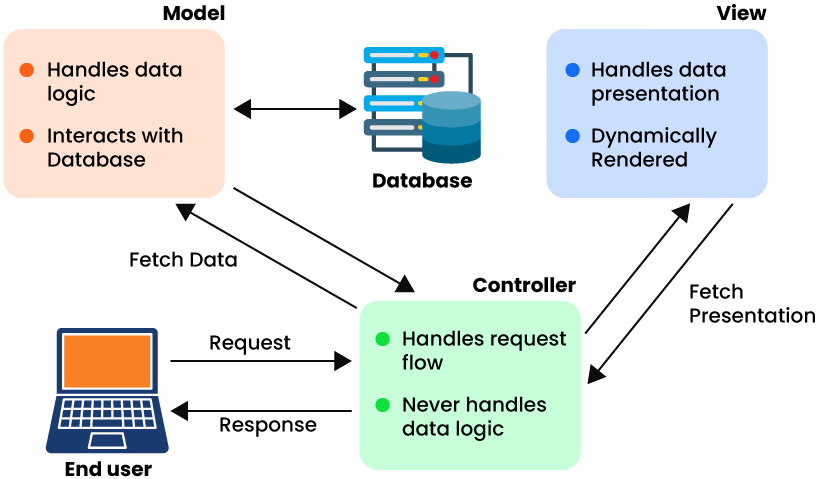
\includegraphics[width=0.4\textwidth]{figures/MVC.png}
\end{figure}

\subsection*{MVVM}
\begin{figure}[H]
   \centering
   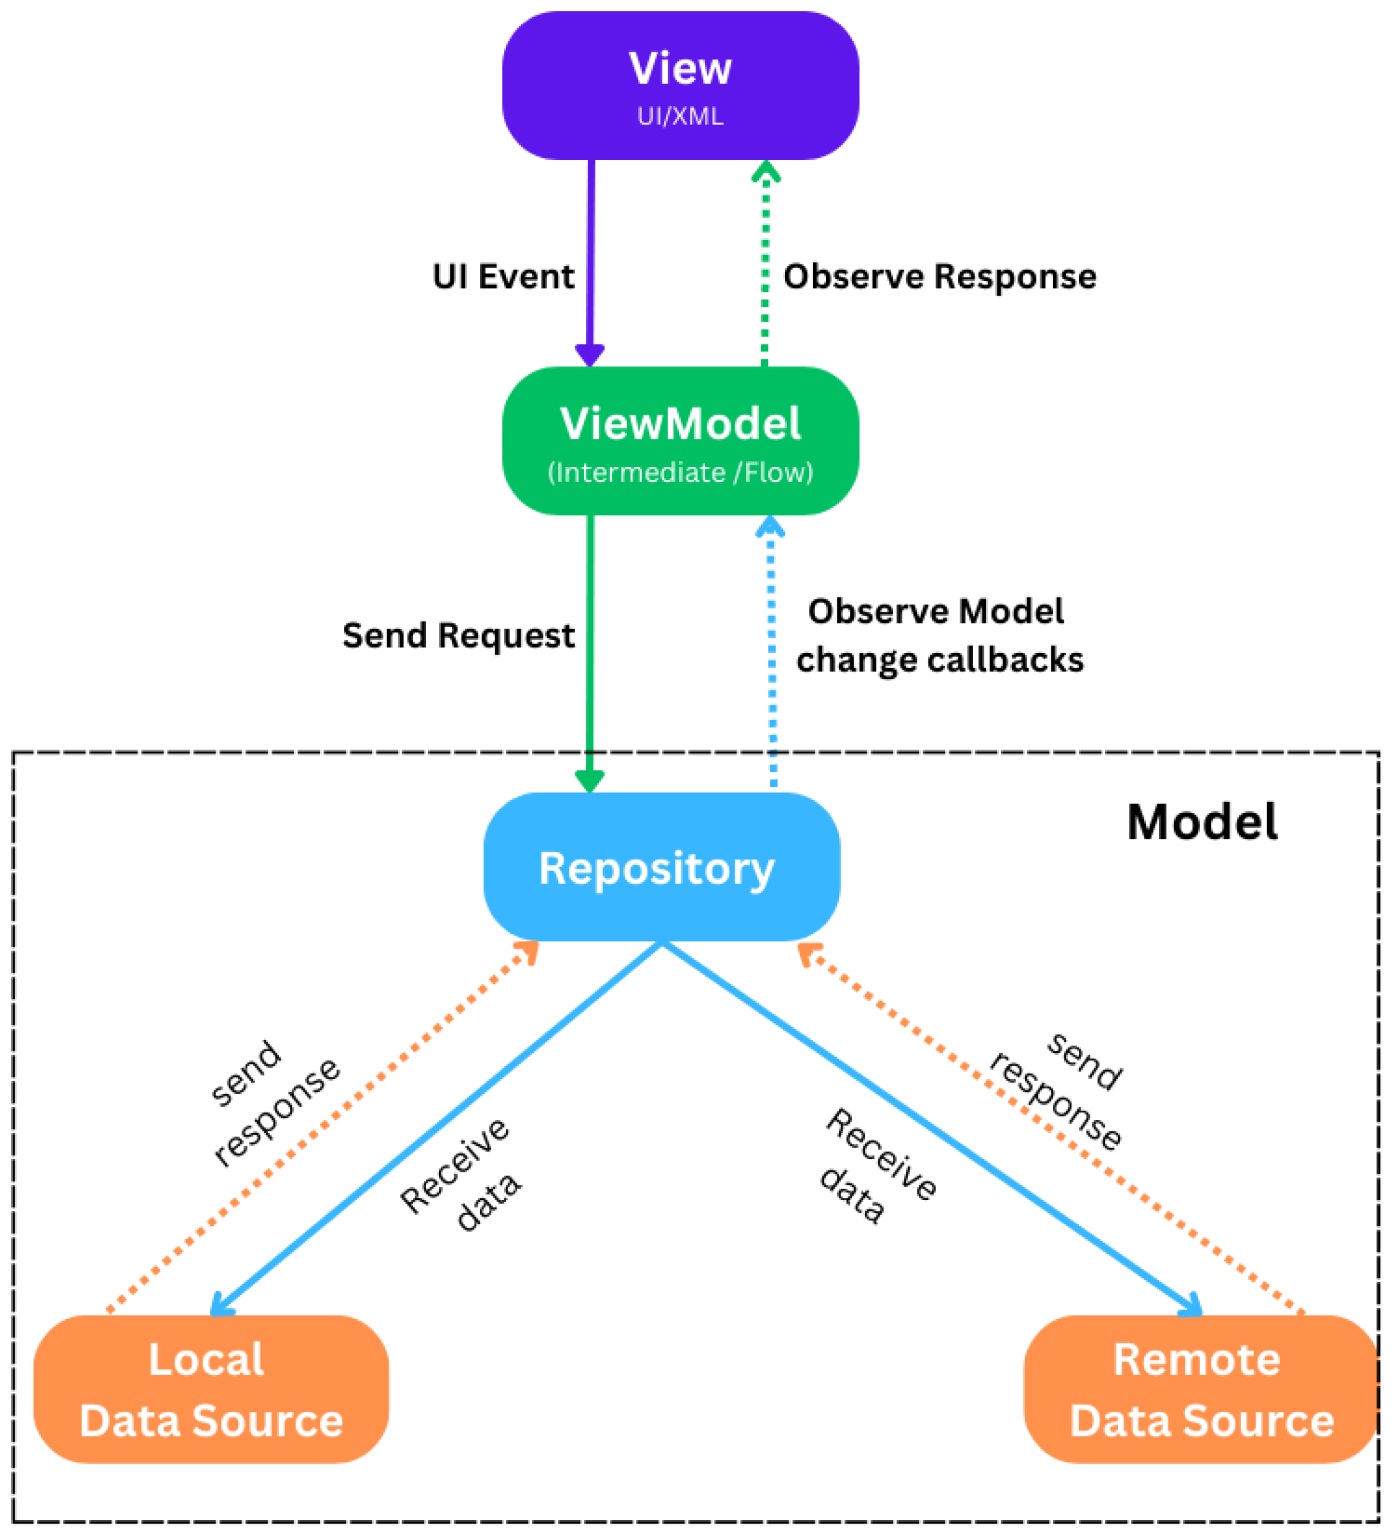
\includegraphics[width=0.4\textwidth]{figures/MVVM.png}
\end{figure}

\subsection*{Layered Architecture}
\begin{figure}[H]
   \centering
   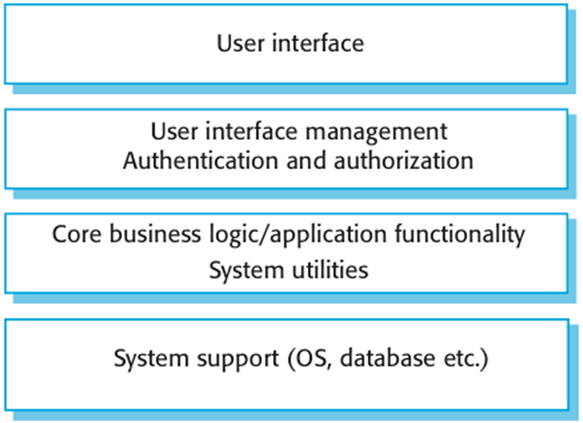
\includegraphics[width=0.4\textwidth]{figures/Layered Architecture.png}
\end{figure}

\subsection*{Client Server Architecture}
\begin{figure}[H]
   \centering
   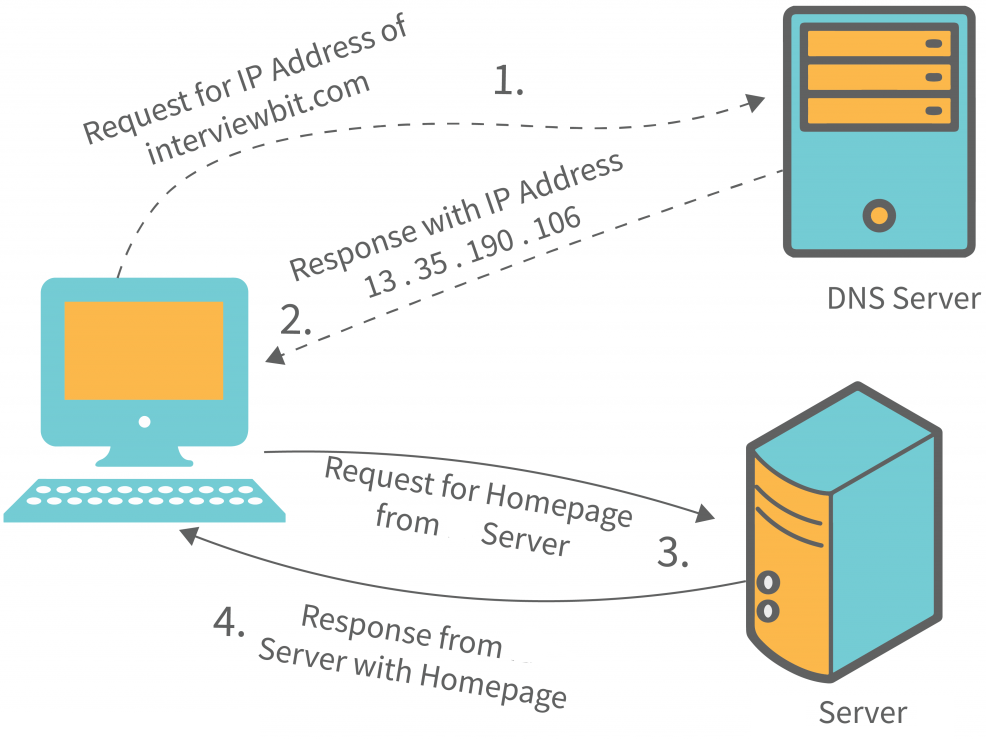
\includegraphics[width=0.47\textwidth]{figures/Client Server.png}
\end{figure}

\vspace{-\baselineskip}
\textbf{Layered Architecture} \gray{|} 3-Tier Architecture
\vspace{-0.5\baselineskip}
\begin{itemize}[parsep=0.25em]
   \item Organizes software into layers, each with specific responsibilities.
   \item Communicates via adjacent layers (top-down or bottom-up)
   \item Scaling individual layers is complex.
   \item Use case: MVC, 3-tier systems
\end{itemize}

\textbf{Client-Server Architecture} \gray{|} 2-Tier Architecture
\vspace{-0.5\baselineskip}
\begin{itemize}[parsep=0.25em]
   \item Organizes system into clients (requesters) and servers (providers).
   \item Communicates over a network (e.g., HTTP, sockets).
   \item Servers/clients can scale independently.
   \item Use case: Web Apps, Cloud Services, Email system
\end{itemize}

\pagebreak
\thispagestyle{empty}
\subsection*{Coupling \& Cohesion}
\textbf{Coupling} \gray{|} Inter-Module Binding
\vspace{-0.5\baselineskip}
\begin{itemize}[parsep=0.15em]
    \item Shows relationships \orange{between modules}
    \item Relative independence between modules should be less
    \item Aim for \orange{low coupling} (minimal dependencies)
    \item Modules are linked to other modules
   \end{itemize}
   
   \textbf{Cohesion} \gray{|} Intra-Module Binding
   \vspace{-0.5\baselineskip}
   \begin{itemize}[parsep=0.15em]
       \item Shows relationship \orange{within a module}
       \item Measures module's functional strength
       \item Aim for \orange{high cohesion} (single function focus)
       \item Module has little interaction with others
       \item Focuses on a single responsibility
\end{itemize}

\subsection*{Dependency Injection}
Dependency Injection is the process of \orange{providing an object (dependency) that a class needs}, rather than letting the class create it itself. Its used to achieve Inversion of Control (IoC) between classes and their dependencies.\\
\textit{Involves four roles:} \blue{Service}, \blue{Client}, \blue{Injector}, and \blue{Interface}.\\
\textit{Ways of DI:} \blue{Constructor}, \blue{Setter}, and \blue{Interface}.


\section*{Verification, Validation \& Testing}

\subsection*{Verification \& Validation}
\textbf{Verification} \gray{|} Static Testing\\[0.2em]
Are we building the product right? \gray{•} Verify product meets design specs. \gray{•} Quality assurance team does verification.
\textbf{Validation} \gray{|} Dynamic Testing\\[0.2em]
Are we building the right product? \gray{•} Ensure product satisfies user needs. \gray{•} Testing team does validation.

\textbf{Cleanroom process} \gray{|} F I S S S\\[0.2em]
\orange{Formal} specification, \orange{Incremental} development, \orange{Structured} programming, \orange{Static} verification, and \orange{Statistical} testing.

\textbf{Inspection process}\\[0.2em]
\textit{Remember:} Please Only Intelligent People In Red Fashion \\[0.25em]
Planning, Overview, Individual, preparation, Inspection, meeting, Rework, and Follow-up

\subsection*{Software testing}
Verifying software correctness by assessing all attributes: reliability, scalability, portability, reusability, and usability. \\[0.5em]
\textbf{\textit{STLC}}: Requirements, Planning, Designing, Setup, Execution, Reporting, and Closure.

\columnbreak
\textbf{Benefits of Software Testing}\\[0.2em]
Cost-Effective, Security, Product Quality, and Customer Satisfaction.

\begin{figure}[H]
      \centering
      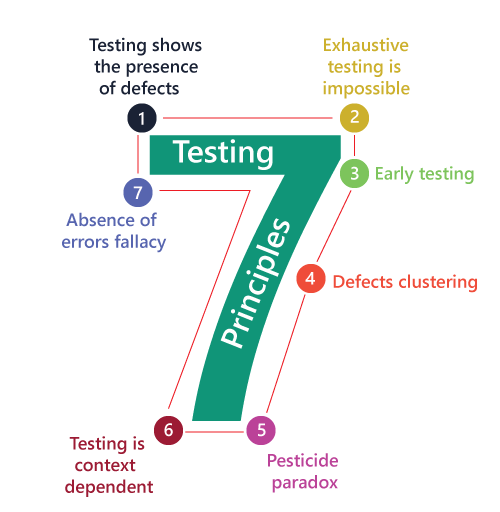
\includegraphics[width=7cm]{figures/Testing Principles.png}
\end{figure}

\textbf{Black box testing} \gray{|} Functional / Behavior Testing\\[0.2em]
Testing software functionality \orange{without looking at internal code}, focusing only on inputs and outputs.\\[0.5em]
\textbf{\textit{Techniques:}} \orange{D}ecision Table, \orange{B}oundary Value, \orange{S}tate Transition, \orange{A}ll-pair Testing, \orange{C}ause-Effect, \orange{E}rror Guessing, and \orange{U}se Case.\\[0.25em]
\textbf{\textit{Generic Steps:}} Requirement Analysis, Test Scenario Design, Test Case Development, Test Execution, Result Comparison, Defect Handling


\textbf{White box testing} \gray{|} Structural / Logic Testing\\[0.2em]
Testing software by looking inside the code, checking logic, conditions, loops, and internal structures.\\[0.5em]
\textbf{\textit{Techniques:}} Statement Coverage, Path Test, Flow Graph Notation, and Loop Testing.


\textbf{Gray box testing} \gray{|} Hybrid Testing\\[0.2em]
Testing with partial knowledge of internal code and user perspective — a mix of black box and white box testing.\\[0.5em]
\textbf{\textit{Techniques:}} Matrix, Pattern, and Regression Testing.


\vspace{4em}
\subsection*{Cost Estimation}
We know that,\\
$E = a(KLOC)^{b} \times EAF$ \quad
$D = c(E)^{d}$ \quad $SS = \frac{E}{D}$ \quad $P = \frac{KLOC}{E}$ \\
Therefore, $EAF \propto E$ 
and $E \propto D$

\begin{tabular}{lllll}
   Experience Level &$\uparrow$ & $EAF$ $\downarrow$
   & E $\downarrow$ & D $\downarrow$\\
   Complexity Level &$\uparrow$ & $EAF$ $\uparrow$
   & E $\uparrow$ & D $\uparrow$\\
   Tools &$\uparrow$ & $EAF$ $\downarrow$
   & E $\downarrow$ & D $\downarrow$
\end{tabular}

   
   
   
\end{multicols}
